% Chapter 2

\chapter{相关工作分析}

本节中,对三种目标检测类别的代表性方法进行分析,并分析了其在CRVC数据集上的局限性及改进方向。此外,本节还将介绍几种利用不同维度、不同来源的数据的方法,详细分析其技术特点,参照其思想,改进CRVC数据集上模型的表现。

\section{目标计数方法分析}
目前目标计数领域主要有三类方法。一类是检测方法\cite{girshick2014rich,girshick2015fast,ren2015faster,redmon2016you,redmon2017yolo9000,he2017mask},通过目标检测模型识别出具体的物体位置,之后根据结果来进一步计数。一种是基于回归的方法\cite{2009BayesianPoissonRegressionCrowdCounting,2013MultisourceMultiscaleCountingExtremelyDenseCrowdImages,2009CrowdCountingUsingMultipleLocalFeatures},直接拟合出图像特征和目标数目之间的回归模型得到图像中对应物体的数目。
另一类方法是基于密度图的目标计数方法\cite{li2018csrnet,2016SingleImageCrowdCountingMultiColumnConvolutionalNeuralNetwork,2018CrowdCountingusingDeepRecurrentSpatialAwareNetwork,2018VehicleDetectionCountingHighResolutionAerialImagesUsingConvolutionalRegressionNeuralNetwork}。此类方法通常先得出一个目标物体在区域内的一个分布,之后就可以通过密度分布来估计总体的数量。
\subsection{YOLO网络}
YOLO(You Only Look Once)
\cite{redmon2016you}是一种广泛应用于实时对象检测任务的深度学习模型。YOLO通过单一的神经网络来预测物体边界和分类概率,从而实现快速且准确的目标检测。

\subsubsection{模型结构}
YOLO模型将对象检测的任务视为一个单一的回归问题,从图像像素直接到边界框的坐标和类别概率。模型的输入是一张图像,输出是一个预测边界框和类别概率的张量。每个预测包含了边界框的四个坐标、一个对象置信度分数以及各类别的概率。YOLO的网络由多个卷积层和汇聚层组成,最后通过一个全连接层输出预测结果。该网络结构能够在整个图像上进行多尺度的特征提取,同时保留足够的空间分辨率以预测小尺寸物体的位置。

在预测时,YOLO将图像划分为一个个格子,每个格子负责预测中心点落在此区域的物体。这样可以使得模型可以同时预测多个位置的多个物体,提升推理效率。每个格子预测多个边界框和相应的置信度分数,置信度分数反映了边界框内存在物体的概率及该边界框的准确性。

在目标计数任务上,YOLO模型通过快速准确的识别出目标锚框并对其计数来得到最终的估计结果。

\subsubsection{局限性}
在通常的计数场景下,计数目标具有清晰的轮廓和准确的真值标注。但是对于CRVC数据集来说,只具有少量具有准确标注的高分辨率图像,大量低分辨率图像中难以分辨出目标具体的位置,也缺少对应的真值标注。由于YOLO依赖于其卷积层来捕捉图像中的特征,但低分辨率图像中的特征捕捉更为困难,因此会导致性能下降。同时CRVC数据集中低分辨率图像的标注不足,可能导致模型训练不充分,从而影响其在实际应用中的准确性和鲁棒性。此外,YOLO虽然能够处理不同尺寸的目标,但对于检测密集分布的低分辨率目标,YOLO的性能往往不是很理想。

因此为了更好的估计低分辨率图像中的目标数目,需要结合场景的先验知识设计专门的网络架构或损失函数,从而提高模型对模糊密集目标的计数能力。

\subsection{贝叶斯泊松回归在人群计数中的应用}
贝叶斯泊松回归\cite{2009BayesianPoissonRegressionCrowdCounting} 是一种在人群计数领域中应用的统计模型。该模型利用泊松分布的特性,对离散计数数据进行建模,并通过引入贝叶斯框架来增强模型的预测性能和鲁棒性。

\subsubsection{模型结构}
贝叶斯泊松回归通过将泊松回归模型扩展到贝叶斯统计框架中,以处理离散数据问题。模型输入为一组特征向量,输出为对应的人数计数,这些计数值被建模为泊松分布的参数。通过引入对于模型参数的先验分布及后验分布估计,对于每一个输入的特征向量,模型预测一个人群计数,并且提供该预测的不确定性度量。

模型采用泊松分布对计数进行建模,其中计数均值是输入特征的线性函数的指数。模型的贝叶斯推理涉及到对参数的后验分布进行估计,通常使用马尔科夫链蒙特卡洛(MCMC)方法或变分推断方法来进行近似计算。

在人群计数的实验中,贝叶斯泊松回归展示了其对复杂场景下人群密度估计的有效性。模型能够准确估计不同场景和时间下的人群数量,对于动态变化的人群场景尤为适用。

\subsubsection{局限性}
该模型在密集物体的计数问题上有着不错的效果,但对于训练数据的要求限制了其在CRVC数据集上的表现。为了降低对高分辨率标注数据的依赖,可以通过半监督或者弱监督学习的方法改进,尤其是利用其余时刻的低分辨率图像进行辅助监督。


\subsection{CRVC网络}
CRVC网络是针对CRVC数据集设计的深度学习模型。该模型将跨分辨率车辆计数问题转换为两个子问题,即综合跨分辨率图像信息的图像分割网络和映射分割结果和最终计数目标的回归模型。它以U-Net模型为骨架,针对跨分辨率空间CRVC数据集中的数据特性设计了两个分支来提取跨分辨率空间信息和时序信息。通过上述网络估计出密度分布后,使用线性回归模型得出最终目标计数结果。

\subsubsection{网络设计}

模型接受4个输入,分别是高分辨率图像输入$I^{HR}$,对应低分辨率图像输入$I^{LR}$,与LR图像时间间隔较近的$I^{LR}_{near}$和与LR图像时间间隔较远的$I^{LR}_{far}$。模型包含两个独立学习的编码器HR encoder和LR encoder,前者用来提取高分辨率图像的特征,后者用来提取3个低分辨率图像的特征。提取出的低分辨率特征和高分辨率特征作差来综合更高精度的信息。之后通过带有跳跃连接的decoder完成分割图的生成。


在CRVC数据集中,车辆在目标区域是密集停放的,而且不存在重叠。因此从分割图上估计出的覆盖率和最终的车辆数目具有线性关系。通过CRVC网络得到的覆盖率分割图,根据低分辨率图像的缩放比例,可以估计出实际面积。通过线性回归,找出参数k来拟合
\begin{equation}
    Number_i=k_i\dots Area_i+b_i
\end{equation}
其中i表示第i类车辆。这些参数通过高分辨率图像的真值计算得到。

\subsubsection{模型局限}
CRVC网络针对CRVC数据集的特点进行了设计,在各项评价指标上均优于传统目标计数方法。然而模型对于样本数量较少的类别的计数效果不是很理想。CRVC网络通过引入两个额外分支来分别提取高分辨率的空间信息和低分辨率的时序信息,然而,对于数据集中的时间连续性和空间一致性信息的挖掘,网络的表现仍有进一步优化的空间。本文针对上述问题进行了针对性设计。



\section{注意力机制及相关方法}
注意力机制(Attention Mechanism)\cite{vaswani2017attention}是一种模仿认知注意力的机制。在认知科学中,由于信息处理的瓶颈,人类会选择性地关注信息中的某一一部分,同时忽略其他可见的信息。上述机制通常被称为注意力机制。随着该机制在Transformer\cite{vaswani2017attention}、BERT\cite{devlin-etal-2019-bert}、GPT\cite{2023GenerativePretrainedTransformerComprehensiveReviewEnablingTechnologiesPotentialApplicationsEmergingChallengesFutureDirections}等NLP领域的成功,该机制及应用又成为了研究的热点话题。目前在计算机视觉领域,ViT\cite{dosovitskiy2021an}、Flow1D\cite{2022ComparisonPoolingMethodsConvolutionalNeuralNetworks}等网络也都基于注意力机制进行设计。
从注意力的形式来分类的话,可以分为软注意力(soft attention)和硬注意力(hard attention)。其中软注意力机制是可微可导的,本文中主要探讨的也是软注意力机制。

\subsection{注意力机制基本原理}

\begin{figure}[h]
  \centering
  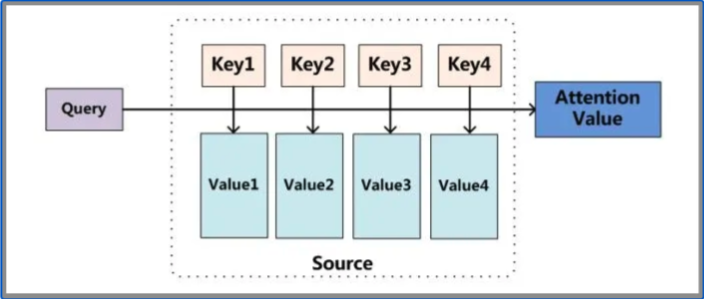
\includegraphics[width=\textwidth]{attention.png}
  \caption{注意力机制}
  \label{fig:attention}
\end{figure}

如图~\ref{fig:attention}所示,注意力机制主要涉及到3类数据,分别是键(key)、值(value)和查询(query)。当一个查询值到来时,计算查询和键的相似度,得到权重,并进行归一化处理。再将得到的权重和值加权求和得到我们最终的注意力结果。
首先计算查询与每个键之间的相似度。这一步通常使用点积(dot product)或者缩放点积(scaled dot product)来实现。具体来说,对于每个查询,通过计算它与所有键的点积,得到一个相似度分数:
\begin{equation}
  \text{score}(Q, K) = QK^T 
\end{equation}

接下来使用Softmax函数对上一步得到的相似度分数进行归一化,以确保所有的权重加起来等于1。:
\begin{equation}
   \text{Attention Weight} = \text{Softmax}(\text{score}(Q, K))
\end{equation}

用归一化后的权重对值进行加权求和,得到最终的注意力输出:
\begin{equation}
  \text{Output} = \text{Attention Weight} \cdot V 
\end{equation}

将上述步骤合并,注意力机制的输出可以通过以下公式计算:
\begin{equation}
\text{Attention}(Q, K, V) = \text{Softmax}\left(\frac{QK^T}{\sqrt{d_k}}\right)V 
\end{equation}

其中,\(d_k\)是键的维度,这个因子用于缩放点积,避免在维度很高时计算结果过大,导致Softmax函数处于饱和区,从而缓解梯度消失的问题\cite{vaswani2017attention}。
\subsection{注意力机制在图像领域的应用}
在图像处理领域中,使用注意力机制可以显著提升模型的性能,尤其是在图像分类、目标检测和图像分割等任务中。根据任务需要不同,常用的注意力机制有以下几种:
\begin{enumerate}    
  \item 空间注意力(Spatial Attention):关注图像的特定区域,通常用于增强模型对图像中重要部分的感知能力。可以用来替代传统的卷积网络,找到目标区域。
  \item 通道注意力(Channel Attention):关注不同通道的相关性,可以帮助模型识别哪些特征是更加重要的。
  \item 自注意力(Self-Attention):通过计算图像内所有位置之间的关系,可以捕捉更广泛的上下文信息。在时间序列模型中,自注意力机制可以保证长序列中的所有位置的信息有参与后续计算的可能。在图像领域中,对图像数据自身使用自注意力机制使得输出中每一位置均含有输入图像中所有位置的加权信息。
\end{enumerate}

在图像领域实践中,同时还使用以下几种训练策略:
\begin{enumerate}    
  \item 多尺度注意力:使用多尺度注意力可以帮助模型同时关注图像的粗略和详细特征,这在处理具有不同尺寸和形状的对象时特别有效。
  \item 融合不同的注意力机制:同时使用空间和通道注意力,或者将传统的注意力机制与自注意力结合起来,可以提取更丰富的特征并提高模型的性能。
  \item 注意力正则化:添加注意力正则化可以防止模型对某些特征过度依赖,从而提高模型的泛化能力。使用如残差连接等设计可以训练更深层的网络,防止训练过程中的信息丢失。
\end{enumerate}

\subsection{注意力机制处理序列图像}
在处理序列图像,如视频帧、时间序列的医学图像或连续的监控遥感数据时,我们不仅要考虑图像中的空间信息,也需要考虑图像间的序列信息。对于注意力机制的设计使用有着更高的要求。自注意力机制和多图像帧的相互注意力机制常常用来捕获时间和空间上的复杂关系。以下是这些注意力机制在序列图像处理中的一些常见应用方式:

自注意力机制可以用于分析序列图像中的时间依赖性,这对于识别视频中的动态事件或时间序列图像中的变化特别有效。
\begin{enumerate}    
  \item 时间自注意力:在处理视频或其他序列图像时,可以在时间维度上应用自注意力,以识别不同时间点图像帧之间的关键依赖关系。在视频帧序列中,模型可以学习到哪些帧之间具有高度相关性,这对于动作识别、事件检测等任务非常有用。
  \item 空间自注意力:在单个图像帧内部,可以应用空间自注意力来分析图像中不同区域之间的相互作用,对于解决目标检测和图像分割等任务有很大的帮助。
  \item 时空自注意力:结合时间和空间自注意力,可以同时考虑空间位置和时间演变的关系。这种方法可以用于复杂场景的动态解析,如多物体交互的场景。
\end{enumerate}

这些方法在处理动态场景解析和增强特征表示上有着不错的表现。在动态变化的场景中,模型可以使用多目标间的相互注意力来预测未来的状态。而通过计算不同目标之间的相互关系,可以获得更丰富的场景表示,这对于场景分类、事件检测等任务非常有帮助。


\subsection{Attention U-Net网络}
Attention U-Net\cite{oktay2018attention}是一种结合了注意力机制的UNet网络,最初被应用于医学图像的分割问题上。它在U-Net的架构上增加了Attention Gate注意力门使得模型能更好的聚焦在目标区域。
\begin{figure}[h]
  \centering
  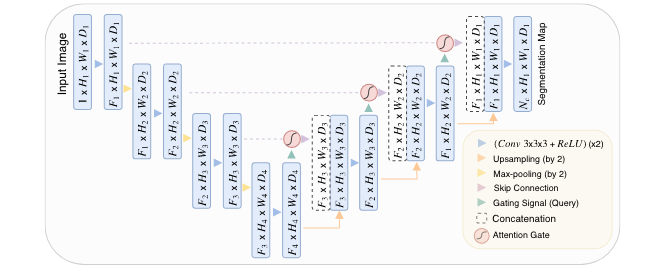
\includegraphics[width=\textwidth]{attention Unet.png}
  \caption{Attention U-Net}
  \label{fig:attentionunet}
\end{figure}

如图~\ref{fig:attentionunet}所示,Attention U-Net沿用了U-Net的基本架构,包括编码器(逐步下采样)和解码器(逐步上采样)两部分,以及跳跃连接(skip connections)来保留多尺度的特征。值得注意的是在每个跳跃连接处,新引入了注意力门控模块。这些模块对来自编码器的特征图进和解码器的相应特征图进行注意力计算。这使得网络能够聚焦于那些对最终分割任务更为重要的区域。

该方法将来自解码器的特征图作为查询,将来自编码器的特征图作为值和键作为注意力门的输入。注意力系数是通过一个小型的卷积网络学习到的,该网络计算当前解码器特征和对应编码器特征之间的相关性。
\begin{figure}[h]
  \centering
  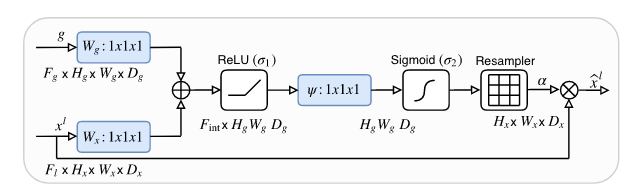
\includegraphics[width=\textwidth]{attention gate.png}
  \caption{Attention gate}
  \label{fig:attentiongate}
\end{figure}


在图~\ref{fig:attentiongate}中展示的是一个注意力门结构。注意力门接收两组输入,一组是来自上一下采样层的特征图(\(g\)),作为查询。另一组是来自跳跃连接的特征图(\(x^l\))键和值。
两组特征图首先通过一个\(1 \times 1 \times 1\)的卷积层(表示为\(W_g\)和\(W_x\)),这一步用于减少通道的数量,以降低后续计算复杂度。
接着,两组卷积后的特征图相加,并通过ReLU激活函数,得到\( \sigma_1\)。经过ReLU激活的特征图再次经过一个\(1 \times 1 \times 1\)卷积层,通常标识为\(\psi\),然后通过Sigmoid激活函数得到\( \sigma_2\),此时每个特征的激活值位于[0, 1]区间,代表了特征的重要性权重。将Sigmoid输出的权重与跳跃连接的特征图(\(x^l\))相乘。在这个过程中,三个\(1 \times 1 \times 1\)卷积层包含了我们需要学习的参数,也赋予了该模块掌握关键权重的能力。通过注意力门,可以得到在解码器特征图做查询的情况下的加权编码器特征图。利用新得到的特征图来进行下一步解码,比原本单纯接受编码器输入获得了更丰富的信息。

本文的模型受此启发,设计了跨分辨率空间注意力和低分辨率下的多来源时空注意力模块,充分综合了不同来源的相关特征信息以提升同一尺度下的分割图生成效果。

\subsection{Flow1D网络}
Flow1D\cite{2022ComparisonPoolingMethodsConvolutionalNeuralNetworks}网络是一个基于注意力机制的光流估计网络。光流估计是计算机视觉中的一个基本问题,它旨在估计一幅图像上的每个像素点在时间序列中的运动,这在视频处理、运动分析、超分辨率、3D重建和自动驾驶等众多领域中都有广泛应用。光流估计是计算机视觉领域中的一个核心问题,光流是图像中像素点在时间维度上的瞬时运动速度和方向的场。光流是从连续的视频帧中估计出来的,这些连续的图像不仅具有时间上的连续性,光流也是从这些图像的空间关系中估计出来的。
\begin{figure}[h]
  \centering
  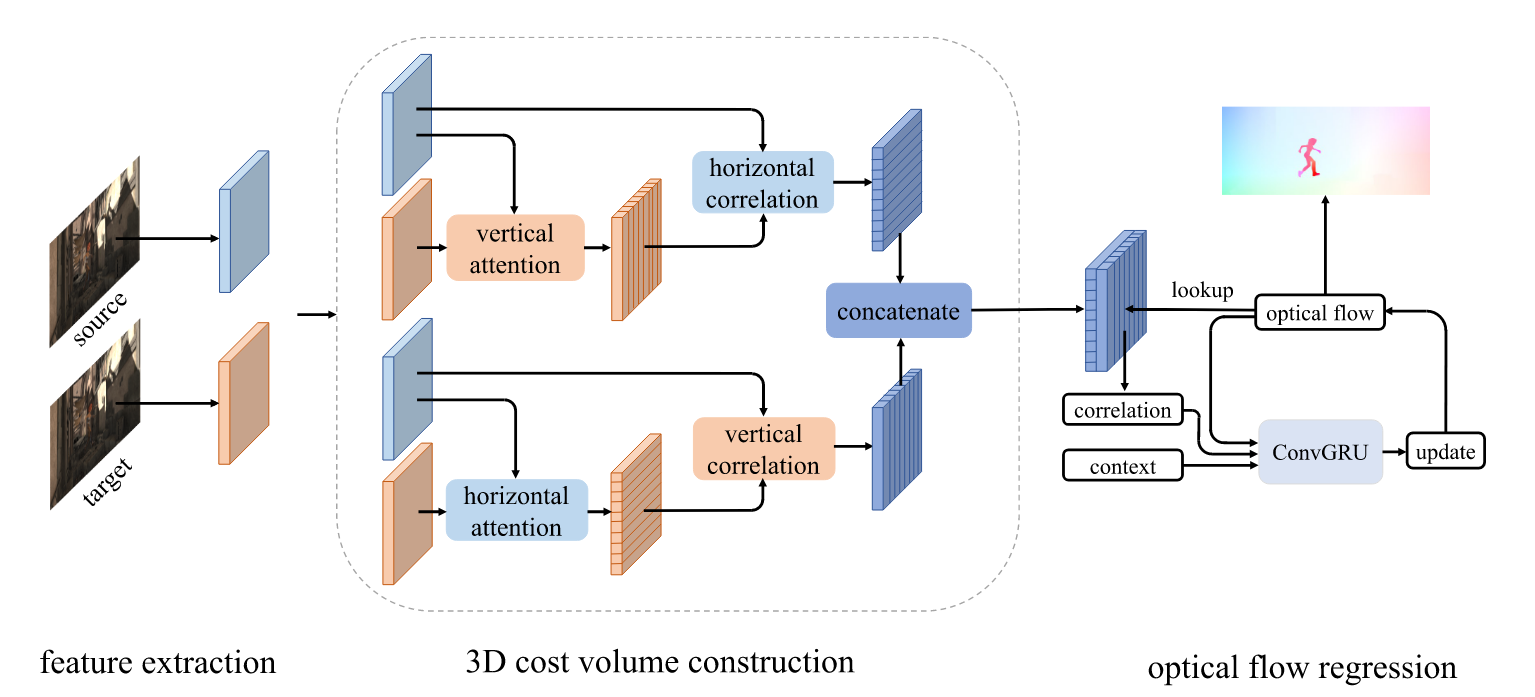
\includegraphics[width=\textwidth]{flow1d.png}
  \caption{Flow1D网络}
  \label{fig:Flow1D}
\end{figure}

图~\ref{fig:Flow1D}展示了模型的基本框架。对于源和目标两个图像,先分别进行特征提取,然后利用注意力机制计算3D cost volume。最后通过门控循环单元,通过相关性特征和初始提取出的特征,进行隐状态的计算。反复迭代计算出光流。
其中3D cost volume的设计充分利用了注意力机制的全局观察能力,通过两个一维的注意力操作,表征三维的光流状态。在水平竖直方向分别进行自注意力计算和相互之间的注意力计算。

\begin{figure}[H]
  \centering
  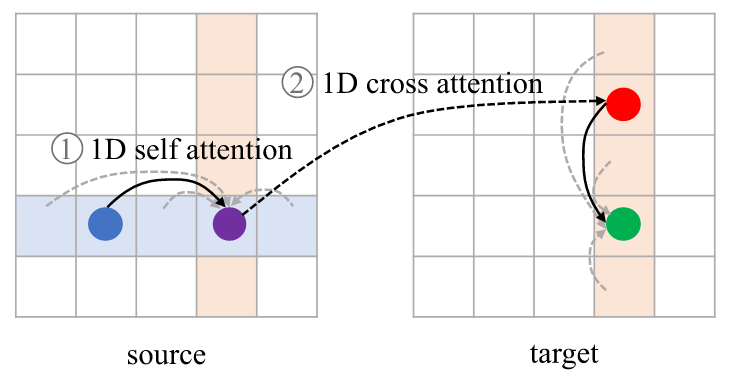
\includegraphics[width=\textwidth]{selfcross.png}
  \caption{self attention和cross attention}
  \label{fig:selfcross}
\end{figure}
图~\ref{fig:selfcross}是对注意力机制的一个很直观的展示。如果要计算源和目标的相关度,直接进行cross attention是不能得到红点与蓝点之间的相关关系的。因此需要再源上先进行self attention,使得每一个列向量包含着原先该列的一种加权分布。然后再进行cross attention操作,综合不同图像不同位置的信息。这是一种非常有效的策略。

本文探讨的跨分辨率车辆计数问题,需要从同一时间的高分辨率图像和低分辨率图像之间找到空间一致性的关联,同时在连续的低分辨率图像中也要找到时间上的连续性关系。这和光流估计对于连续图像数据的利用有着不少相同之处。


